\section{Does look-ahead raise the reward?}
\label{sec:reward}

\begin{figure*}[t]
  \centering
  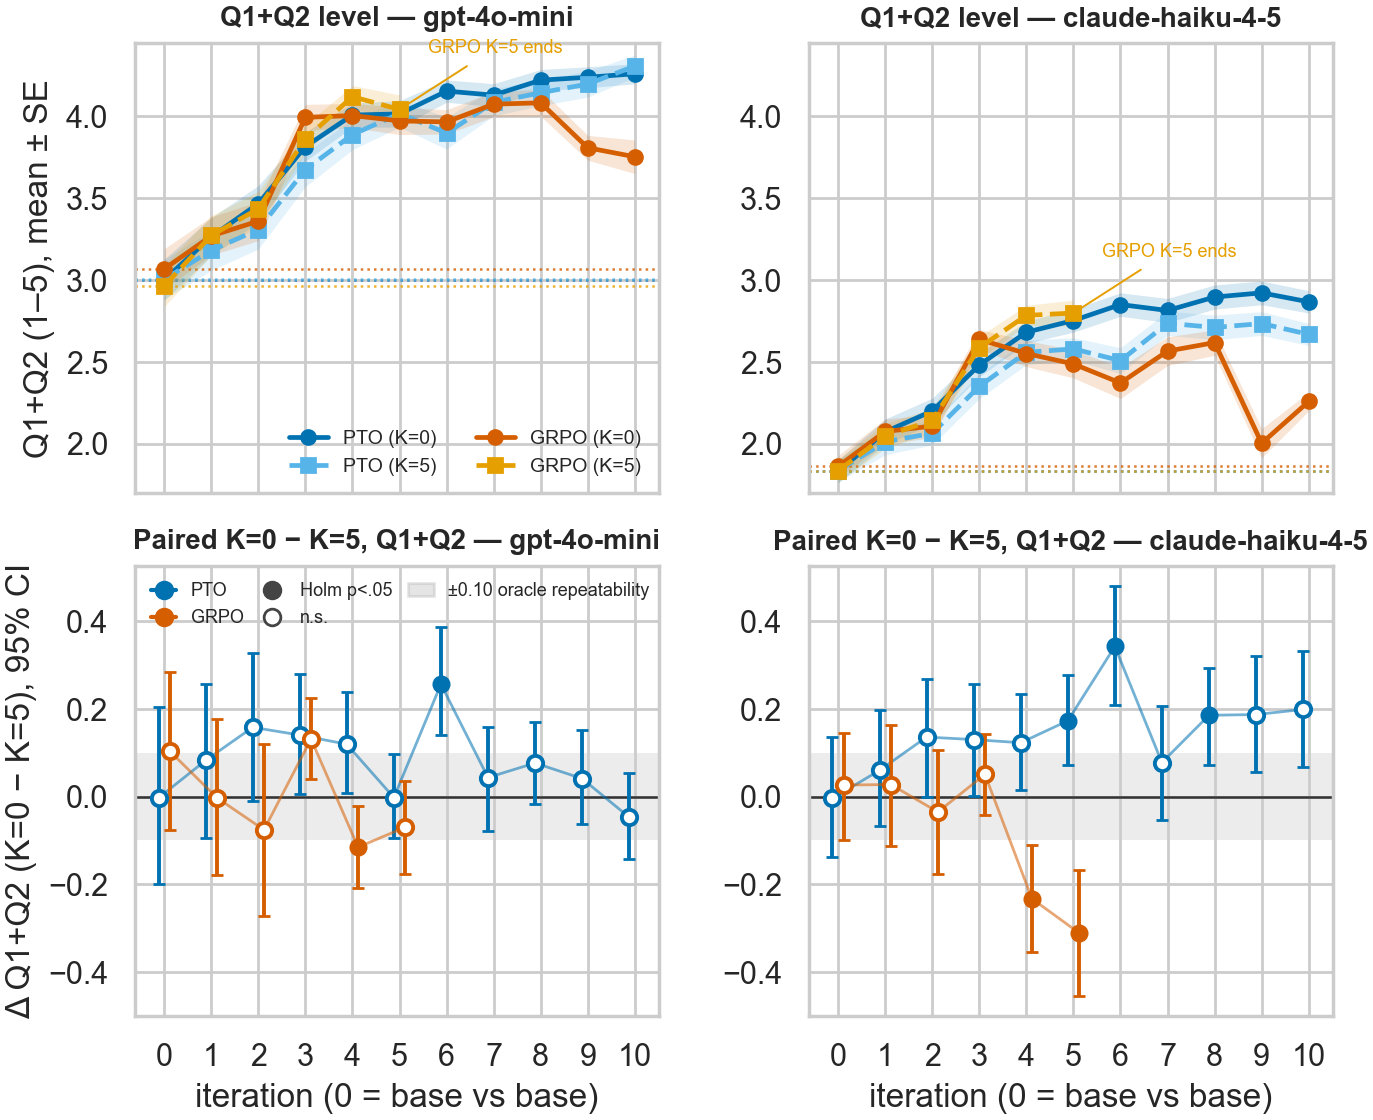
\includegraphics[width=0.85\textwidth]{figures/k_contrast_headline_fig_q1q2.png}
  \caption{\QQ{} under the training oracle (\primaryjudge{}, left) and the held-out judge
    (\heldoutjudge{}, right). Top: level by iteration, mean $\pm$ SE over 96 personas (dotted: base;
    GRPO \Kf{} ends at 5). Bottom: persona-paired $K{=}0$ minus $K{=}5$, 95\% bootstrap CI
    (positive $=$ \Kz{} higher); filled $=$ Holm-significant across iterations; grey band $=$
    $\pm 0.10$ repeatability.}
  \label{fig:headline}
\end{figure*}

\begin{table}[t]
  \centering\scriptsize
  \setlength{\tabcolsep}{2.5pt}
  \begin{tabular}{@{}c rr rr@{}}
    \toprule
    & \multicolumn{2}{c}{PTO} & \multicolumn{2}{c}{GRPO} \\
    \cmidrule(lr){2-3}\cmidrule(lr){4-5}
    iter. & oracle & held-out & oracle & held-out \\
    \midrule
    0  & $-.003$ (.00) & $-.004$ (.01) & $+.104$ (.11) & $+.026$ (.04) \\
    1  & $+.083$ (.09) & $+.060$ (.09) & $-.003$ (.00) & $+.028$ (.04) \\
    2  & $+.158$ (.18) & $+.136$ (.20) & $-.076$ (.08) & $-.035$ (.05) \\
    3  & $+.141$ (.20) & $+.130$ (.20) & $+.132$ (.28) & $+.051$ (.11) \\
    4  & $+.120$ (.20) & $+.123$ (.21) & $-.115$ (.25)$^{*}$ & $-.233$ (.37)$^{**}$ \\
    5  & $-.002$ (.00) & $+.173$ (.33)$^{*}$ & $-.070$ (.13) & $-.311$ (.43)$^{**}$ \\
    6  & $+.257$ (.42)$^{***}$ & $+.343$ (.51)$^{***}$ & --- & --- \\
    7  & $+.044$ (.07) & $+.078$ (.12) & --- & --- \\
    8  & $+.077$ (.17) & $+.186$ (.34)$^{**}$ & --- & --- \\
    9  & $+.041$ (.08) & $+.187$ (.29) & --- & --- \\
    10 & $-.047$ (.10) & $+.199$ (.31) & --- & --- \\
    \bottomrule
  \end{tabular}
  \caption{Persona-paired $K{=}0$ minus $K{=}5$ on \QQ{} by iteration: mean difference ($|\dz|$),
    $n{=}96$; positive $=$ \Kz{} higher. Stars: Holm across iterations 0--$N$ within (grader,
    method); ${}^{*}p{<}.05$, ${}^{**}p{<}.01$, ${}^{***}p{<}.001$. Iteration~0 is two independent
    base draws. GRPO \Kf{} is censored at iteration~5.}
  \label{tab:kcontrast}
\end{table}

Throughout, a contrast is $K{=}0$ minus $K{=}5$: positive means the arm \emph{without}
look-ahead scores higher.

\paragraph{PTO: look-ahead does not raise the reward.} Under the training oracle the \Kz{} arm
is at or above \Kf{} at eight of ten trained iterations, is never significantly below it, and is
significantly above it once, at iteration~6 ($+0.257$, \dz{} $0.42$, $p_{\text{Holm}}{=}.001$;
Table~\ref{tab:kcontrast}, Figure~\ref{fig:headline}). The held-out judge sees the same edge as larger and more persistent:
\Kz{} is higher at all ten iterations, Holm-significantly at 5, 6 and 8 ($+0.173$/\dz{} $0.33$, $+0.343$/$0.51$,
$+0.186$/$0.34$). At the endpoint the contrast is null under the training oracle ($-0.047$,
\dz{} $-0.10$) and $+0.199$ (\dz{} $0.31$, CI $[0.068, 0.332]$, not Holm-significant) under the
held-out judge (Table~\ref{tab:app:endpoints}). The edge is carried by Q2, the working-alliance rubric: held-out Q2 favours \Kz{}
at iterations 5--10 (\dz{} $0.33$--$0.65$, all Holm-significant) while held-out Q1 does so only
at iteration~6; the training oracle's Q2 is significant at 6 ($+0.341$, \dz{} $0.52$) and 8
($+0.145$, \dz{} $0.33$) and its Q1 never is --- the poster's one significant sub-scale, with the
sign reversed.

\paragraph{GRPO: the sign flips, on Q1.} No GRPO contrast clears Holm correction before
iteration~4 under either grader (the base pair already differs by $+0.104$ under the training
oracle, $+0.026$ under the held-out judge). From iteration~4
the \Kf{} arm is higher: $-0.115$ (\dz{} $-0.25$, $p_{\text{Holm}}{=}.044$) at
iteration~4 and $-0.070$ (n.s.) at 5 under the training oracle; $-0.233$ (\dz{} $-0.37$) and
$-0.311$ (\dz{} $-0.43$), both $p_{\text{Holm}}{=}.006$, under the held-out judge. This is a Q1
effect: at iteration~5 held-out Q1 is $-0.450$ (\dz{} $-0.50$, $p_{\text{Holm}}{<}.001$)
against Q2 $-0.172$ (n.s.). GRPO \Kf{} is censored at iteration~5, so the reversal is measured and its
persistence is not.

\paragraph{The interaction.} At iteration~5 the method gap depends on $K$: under the held-out judge PTO leads GRPO by $+0.265$ (\dz{} $0.36$) at \Kz{} and
trails it by $-0.219$ (\dz{} $-0.38$) at \Kf{}, a persona-level difference-in-differences of
$+0.484$ (\dz{} $0.52$, CI $[0.307, 0.675]$, $p_{\text{Holm}}{<}.001$ across iterations and
across instruments alike). Under the
training oracle the same quantity is $+0.068$ (\dz{} $0.10$, n.s.). The optimizer that ``wins''
flips with $K$ --- but one grader sees it and the other does not (Table~\ref{tab:app:did},
Figure~\ref{fig:did}).

\paragraph{What transfers to the held-out judge.} Gain retention is the held-out gain over an
arm's own base divided by the oracle gain over the same base: how much of what the oracle
rewarded a second grader also sees. For GRPO at iteration~5 the ordering favours \Kf{} but is
reference-dependent: \Kf{} retains its full Q1 gain ($1.05$, CI $[0.91, 1.22]$) against \Kz{}'s
$0.79$ ($[0.59, 1.00]$), yet the intervals overlap under own bases and separate only when the
\Kf{} arm's base is the shared reference ($1.05$ vs $0.71$ $[0.54, 0.88]$; under the \Kz{} arm's
base they still touch, $1.16$ $[0.99, 1.39]$ vs $0.79$ $[0.59, 1.00]$), and the two GRPO base
draws differ by $0.104$ on \QQ{} ($0.110$ on Q1), so we report the range.
For PTO at iteration~10 the ordering is reversed and reference-robust: \Kf{} retains less of
its Q2 gain ($0.56$ $[0.48, 0.65]$ vs $0.85$ $[0.75, 0.98]$) and its MITI gain ($0.27$
$[0.18, 0.35]$ vs $0.45$ $[0.36, 0.55]$), both disjoint (Table~\ref{tab:app:retention}). Over
all 153 cross-$K$ contrasts (17 iteration pairs $\times$ 9 instruments;
Table~\ref{tab:app:summary}, Figures~\ref{fig:grid:primary}--\ref{fig:grid:heldout}) the
held-out judge keeps the oracle's sign in $18/18$ cases where the oracle is Holm-significant;
what it changes is how large the gap is and which optimizer it favours.
